\documentclass[aps,prb,reprint,groupedaddress,showpacs,amsfonts,amsmath,amssymb,superscriptaddress]{revtex4-1}
\usepackage{graphicx}
% \usepackage{subfigure}
\usepackage{bm}
\usepackage{color}
% \usepackage{changes}
    % \definechangesauthor[name={Wang Shi}, color=orange]{swang}

\usepackage[colorlinks,urlcolor=blue,linkcolor=blue,anchorcolor=blue,citecolor=blue,bookmarks]{hyperref}

\begin{document}

\title{Global phase diagram and possible quantum spin liquid in the triangular $J-K-\Gamma$ model}

\author{Shi Wang}
\affiliation{National Laboratory of Solid State Microstructures and School of Physics, Nanjing University, Nanjing 210093, China}
\author{Shun-Li Yu}
\email{slyu@nju.edu.cn}
\affiliation{National Laboratory of Solid State Microstructures and School of Physics, Nanjing University, Nanjing 210093, China}
\affiliation{Collaborative Innovation Center of Advanced Microstructures, Nanjing University, Nanjing 210093, China}
\author{Jian-Xin Li}
\email{jxli@nju.edu.cn}
\affiliation{National Laboratory of Solid State Microstructures and School of Physics, Nanjing University, Nanjing 210093, China}
\affiliation{Collaborative Innovation Center of Advanced Microstructures, Nanjing University, Nanjing 210093, China}

\date{\today}

\begin{abstract}
    The global ground state phase diagram of the Heisenberg-Kitaev-$\Gamma$ model on a triangular lattice is studied using classical Monte Carlo and exact diagonalization. \textcolor{red}{$\cdots \cdots$}
\end{abstract}

\maketitle

\section{Introduction}
Geometric frustration, which arises when the lattice geometry gives rise to constraints that cannot be simultaneously satisfied, plays an important role in various kinds of magnetic systems. In particluar, antiferromagnets on the triangular lattice are typical examples of such geometric frustated spin systems and have attracted numerous interests in condensed matter physics. For nearest-neighbor (NN) spin-$1/2$ antiferromagetic Heisenberg model on triangular lattice, though a fully disordered resonating-valence-bond (RVB) \cite{Anderson1973} state was proposed as the possible ground state in the early years, several studies point to a 120$^\circ$ N\'{e}el-ordered ground state thereafter \cite{PhysRevLett.99.127004,PhysRevLett.82.3899,PhysRevB.50.10048,PhysRevLett.60.2531}. When the second NN interactions are included which introduce further frustration, the system has a much richer phase diagram including a N\'{e}el phase, a phase with spin-wave selection of nontrivial ground states and a phase with incommensurate long-range order \cite{PhysRevB.42.4800,PhysRevB.46.11137}. All these studies have revealed that geometric frustated systems show quite different behavior from that of the non-frustated system.

On the other hand, exchange frustation in systems with strongly anisotropic magnetic interactions has been shown to be another promising approach to explore exotic quantum spin states. Like geometric frustation, the effect of exchange frustration is to prevent the formation of long range magnetic order and given raise to a residual ground-state entropy. The spin-$1/2$ Kitaev model \cite{Kitaev2006} on honeycomb lattice, which has both gapped and gapless quantum spin liquid (QSL) ground state (GS) supporting fractionalized excitations, is an example of a model with exchange frustration. As pointed out by Jackeli and Khaliullin \cite{Khaliullin2005, PhysRevLett.102.017205}, the elementary ingredients for realizing this highly anisotropic spin model are strong relativistic spin-orbit coupling (SOC), electron interactions, and specific geometric structure: edge sharing octahedra with 90$^\circ$ TM-O-TM bond angles. Because of its theoretical importance and potential application in quantum computing, great efforts have been made to search a solid-state realization of the Kitaev model. It was first proposed to be realized in iridates $A_2$IrO$_3$ (A = Na or Li) \cite{PhysRevLett.105.027204,PhysRevLett.108.127204,Chun2015,PhysRevLett.110.076402,PhysRevB.87.220407,PhysRevLett.110.097204,PhysRevLett.108.127203,PhysRevB.92.024413,PhysRevLett.112.077204,Rau2014}, and then turned towards $\alpha$-RuCl$_3$ \cite{PhysRevB.91.180401,Banerjee2016,PhysRevB.92.235119,PhysRevB.94.161106,PhysRevB.93.214431,PhysRevLett.118.107203,PhysRevLett.118.107203,PhysRevB.96.115103} in which Ir$^{4+}$/Ru$^{3+}$ ions are arranged in a honeycomb lattice and carry effective $j_{eff}=1/2$ moments. In fact, magnetic ions located at the center of edge-shared octahedra can not only form honeycomb lattice, but also triangular lattice and the Kitaev term can naturally be generalized to this scenario \cite{PhysRevB.93.104417,PhysRevB.89.014414}. Moreover, the symmetric off-diagonal $\Gamma$ term is allowed by symmetry and is a generic feature of S=$1/2$ models with edge sharing octahedra \cite {PhysRevLett.112.077204}. Kai Li \emph{et al.,} \cite{KaiLi2015} have studied the Heisenberg-Kitaev (HK) model on triangular lattice and a global phase diagram with a mean-field level chiral spin liquid (SL) as well as four magnetically ordered phases has been obtained. However, the effect of the $\Gamma$ term on triangluar lattice has not gain as much attention as on honeycomb lattice \cite{PhysRevLett.112.077204,Rau2014,PhysRevLett.118.107203,PhysRevB.96.115103,PhysRevB.93.214431,PhysRevB.100.144422}.

On the experimental side, the discovery of YbMgGaO$_4$ has invoked increasing interest in searching for rare-earth based spin-frustrated materials \cite{srep16419,PhysRevLett.115.167203,PhysRevB.94.035107,PhysRevB.96.054445,PhysRevB.97.184413,PhysRevB.97.125105,PhysRevB.96.075105,PhysRevLett.119.157201}. The Yb$^{3+}$ ions form a triangular layer and are surrounded by O$^{2-}$ which construct edge sharing octahedra \cite{srep16419,PhysRevLett.115.167203}. Extensive studies of magnetic properties using neutron scattering \cite{Nature20614,nphys3971,PhysRevLett.117.267202,PhysRevX.8.031001}, muon spin relaxation ($\mu$SR) \cite{PhysRevLett.117.097201}, electron spin resonance (ESR) \cite{PhysRevLett.115.167203} reveal a possible gapless quantum spin liquid (QSL) ground state. More recently, a class of compounds \emph{AReCh}$_2$ (A=alkali, Re=rare-earth, Ch=O, S, Se) with perfect triangular lattices of rare-earth ions have been synthesized and explored. The magnetic susceptibilty and heat capacity data suggest no long-range magnetic order or spin freezing down to the lowest measurement temperature, which implies their candidacy for QSL state \cite{acsmaterialslett.9b00464,PhysRevMaterials.3.114413,arXiv1911.08036,Liu_2018,arXiv1911.12712}. The novel magnetic properties of these triangluar magnets may be attributed to the interplay of geometric frustation and exchange frustration induces by spin-orbit coupling.

Inspired by previous theoretical and experimental works, we study the Heisenberg-Kitaev-$\Gamma$ ($J-K-\Gamma$) model on the triangular lattice. The $J-K-\Gamma$ model Hamiltonian is given by
\begin{equation}
    H=\sum_{\langle i,j \rangle \in \alpha \beta (\gamma)} \lbrack J \bm{S}_i \bm{\cdot} \bm{S}_j + K S_i^{\gamma} S_j^{\gamma} + \Gamma (S_i^{\alpha} S_j^{\beta} + S_i^{\beta} S_j^{\alpha}) \rbrack
\end{equation}
where $\langle i,j \rangle$ denotes the NN bonds, $\gamma$ takes value $x$, $y$, or $z$ depending on the direction of the NN bond as shown in Fig. 1, and $\alpha$, $\beta$ are the remaining directions. $J$ and $K$ are the magnitude of the Heisenberg and Kitaev interactions and $\Gamma$ the symmetric off-diagonal exchanges. To the best of our knowledge, no exact solution has been reported so far for the spin-$1/2$ Kitaev and/or $\Gamma$ model on the triangular lattice. Therefore, it remains conceptually interesting to investigate whether the QSL could exist as a possible ground state of the triangular $J-K-\Gamma$ model.

In this manuscript, by combining the classical Monte Carlo simulation and exact diagonalization (ED) calculation, we map out the global phase diagram of the $J-K-\Gamma$ model. \textcolor{red}{$\cdots\cdots$}

The rest of the paper is organized as follows: \textcolor{red}{$\cdots\cdots$}

\begin{figure}
    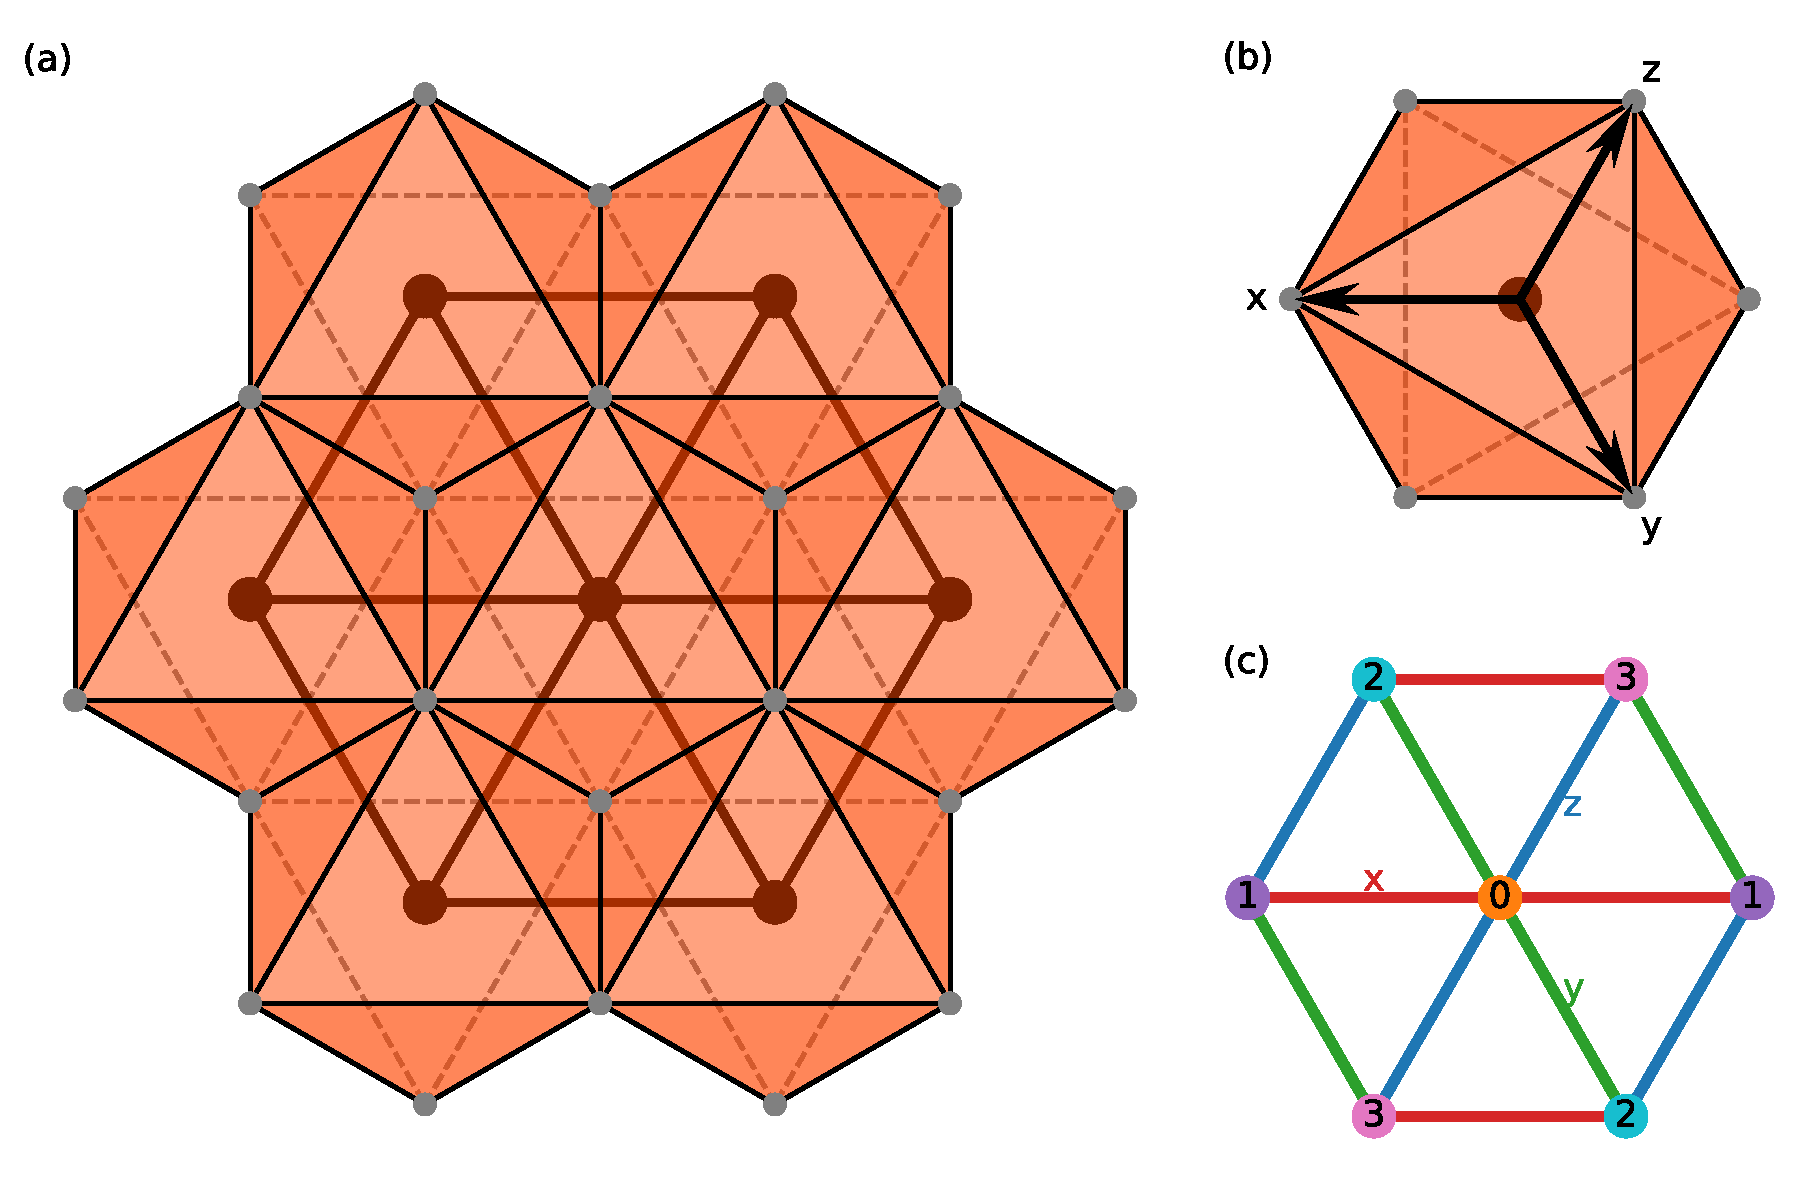
\includegraphics[width=0.45\textwidth]{Fig1.pdf}
    \caption{(Color online) (a) Top view of the triangular lattice of the edge-sharing octahedral. (b) Three different direction of the NN bonds on the triangular lattice, namely $\gamma=x, y, z$ colored red, green and blue respectively. The different colors of the lattice sites label the four sublattices realizing the four-sublattice-transformation. (c) The orientation of the cubic $x$, $y$, $z$ with respect to the octahedral. The spin operators $S^x$, $S^y$ and $S^z$ are defined with respect to this reference frame.}
     \label{fig:ModelDefinition}
\end{figure}

\section{Methods}

The ground state of the full anisotropic Hamiltonian is no longer solvable in closed analytical form, even in the classical case. One, therefore, either has to rely on approximate analytical method or on numerical techniques. Here, we briefly describe the methods we used. \textcolor{red}{$\cdots\cdots$}

\subsection{Dual Transformation}
\textcolor{red}{A introduction to dual transformation. Left blank currently.}

\subsection{Classical Monte Carlo}
\textcolor{red}{A introduction to classical Monte Carlo. Left blank currently.}

\subsection{Exact Diagonalization}
\textcolor{red}{A introduction to exact diagonalization. Left blank currently.}

\section{Phase Diagram and Analysis}
\textcolor{red}{Global phase diagram of the $J-K-\Gamma$ model. Left blank currently.}

\begin{figure*}
    \centering
    % \subfigure{\includegraphics[width=0.96\textwidth]{Fig2_a.pdf}}\\
    % \subfigure{\includegraphics[width=0.96\textwidth]{Fig2_b_f.pdf}}\\
    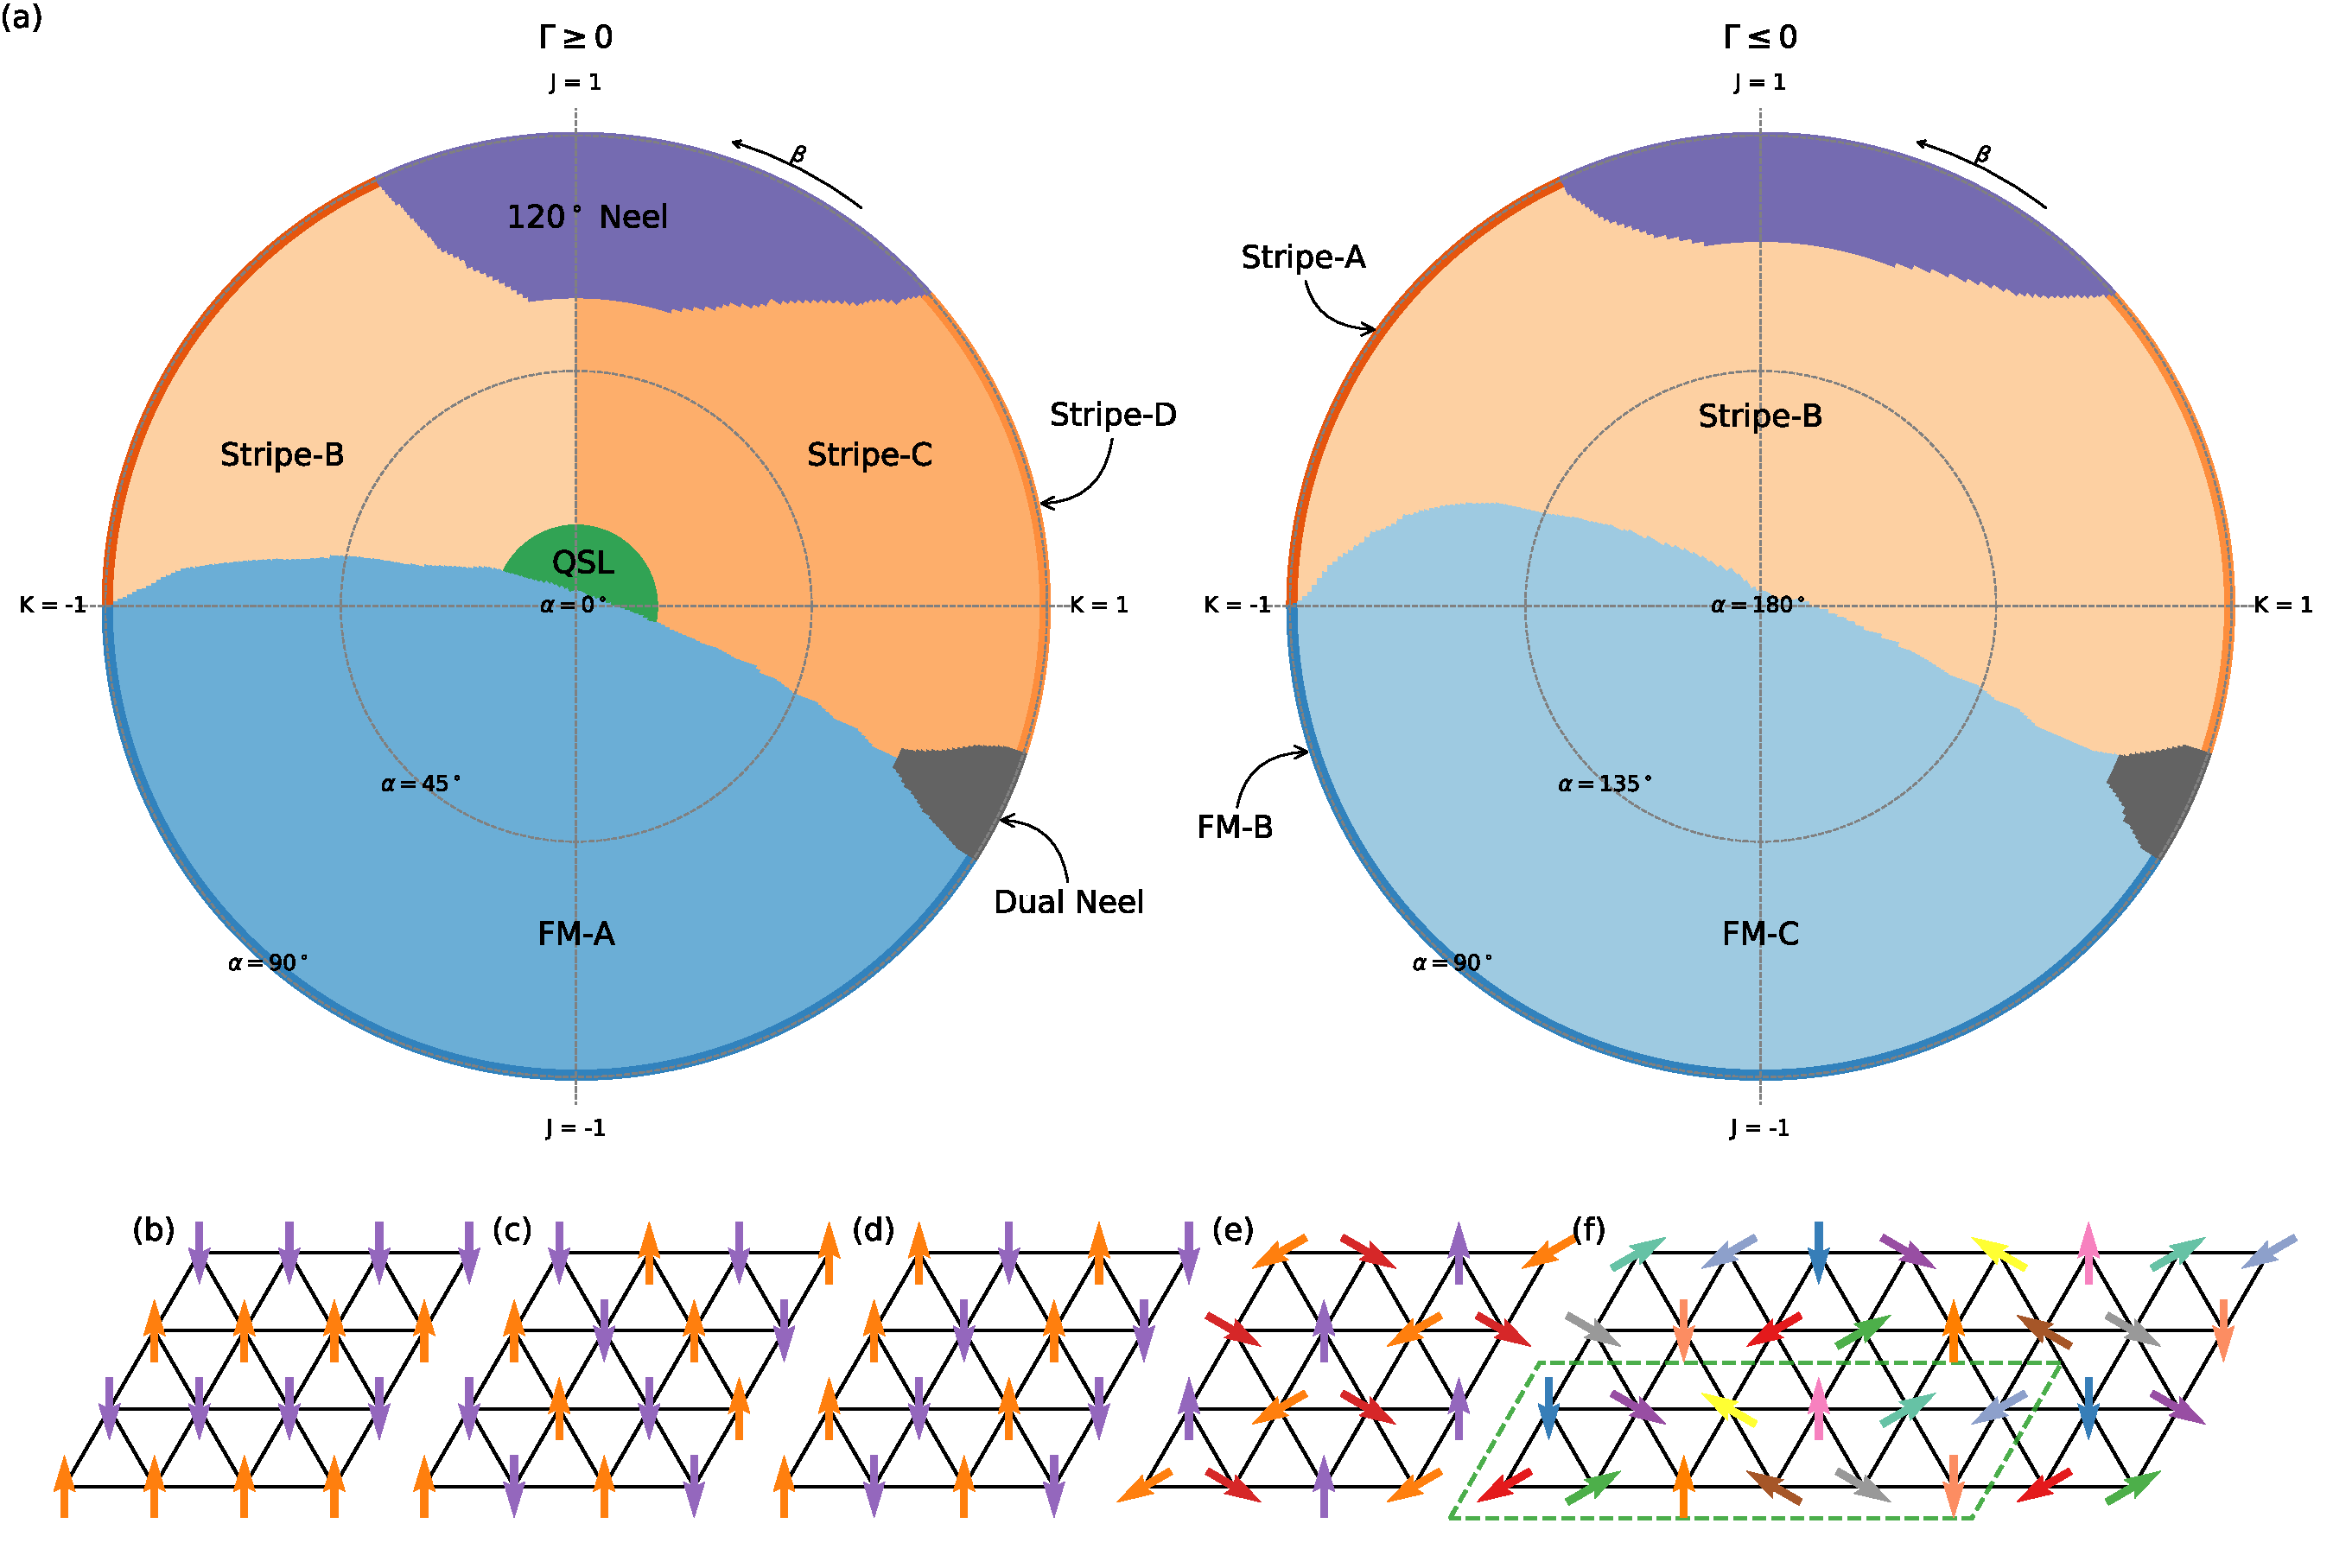
\includegraphics[width=0.96\textwidth]{Fig2.pdf}
    \caption{(Color online) (a) Global phase diagram of the triangular lattice J-K-$\Gamma$ model. The angle $\alpha$ and $\beta$ denote the radial and azimuthal angles, respectively. There are in total ten phases including three different FM phases denoted as FM-A, FM-B and FM-C, four different stripe phases designated as Stripe-A, Stripe-B, Stripe-C and Stripe-D, 120$^\circ$ N\'{e}el, Dual N\'{e}el and a possible quantum spin liquid phase. (b) Illustration of the FM order. All spins along the same direction. (c) Illustation of the stripe order of the $x$ type. That is the spins along the x-bond direction are parallel and adjacent chains are antiparallel. There are also stripe order of the $y$ or $z$ type, which are degenerate with the $x$ type stripe order. (d) Illustration of the 120$^\circ$ N\'{e}el order. All spins are coplanar and the angles between nearest-neighbor spins are 120$^\circ$. (e) Illustration of the Dual N\'{e}el order. The magnetic unit cell include 12 lattice sites as marked by the green dashed parallelogram.}
     \label{fig:PhaseDiagram}
\end{figure*}

\begin{figure}
    \includegraphics[width=0.45\textwidth]{Fig3.pdf}
    \caption{(Color online) Static structure factors for different model paramters.}
     \label{fig:StructureFactors}
\end{figure}

\begin{figure}
    \includegraphics[width=0.45\textwidth]{Fig4.pdf}
    \caption{(Color online) Map of the probabilities.}
     \label{fig:StructureFactors}
\end{figure}

\section{Discussion}
\textcolor{red}{A discussion of our results. Left blank currently.}

\section{Acknowledgements}
\textcolor{red}{Acknowledgements. Left blank currently.}

\bibliography{ref}

\end{document}
